\documentclass[12pt]{article}
\usepackage{amsthm,amssymb,amsmath,amsfonts}
\usepackage[a4paper, top=25mm, bottom=30mm, left=25mm, right=25mm]{geometry}
\usepackage[pagebackref=false,colorlinks,linkcolor=black,citecolor=black]{hyperref}
\usepackage[nameinlink]{cleveref}
 \AtBeginDocument{%
    \crefname{equation}{برابری}{equations}%
    \crefname{chapter}{فصل}{chapters}%
    \crefname{section}{بخش}{sections}%
    \crefname{appendix}{پیوست}{appendices}%
    \crefname{enumi}{مورد}{items}%
    \crefname{footnote}{زیرنویس}{footnotes}%
    \crefname{figure}{شکل}{figures}%
    \crefname{table}{جدول}{tables}%
    \crefname{theorem}{قضیه}{theorems}%
    \crefname{lemma}{لم}{lemmas}%
    \crefname{corollary}{نتیجه}{corollaries}%
    \crefname{proposition}{گزاره}{propositions}%
    \crefname{definition}{تعریف}{definitions}%
    \crefname{result}{نتیجه}{results}%
    \crefname{example}{مثال}{examples}%
    \crefname{remark}{نکته}{remarks}%
    \crefname{note}{یادداشت}{notes}%
    \crefname{observation}{مشاهده}{observations}%
    \crefname{algorithm}{الگوریتم}{algorithms}%
    \crefname{cproof}{برهان}{cproofs}%
}

\usepackage{tikz}
\usepackage{graphicx}
\usepackage{color}

\usepackage{setspace}
\doublespacing
\usepackage{listings}

\lstnewenvironment{code}[1][]%
  {\minipage{\linewidth} 
   \lstset{basicstyle=\ttfamily\footnotesize,frame=single,#1}}
  {\endminipage}
  
\usepackage{titletoc}
\usepackage{tocloft}
\usepackage{enumitem}
\usepackage{lipsum} % for dummy text
\usepackage{tikz}
\usepackage{eso-pic}

\AddToShipoutPictureBG{% Add picture to background of every page
    \begin{tikzpicture}[remember picture,overlay]
    \draw[line width=1pt]
        ([shift={(1cm,-1cm)}]current page.north west)
        rectangle
        ([shift={(-1cm,1cm)}]current page.south east);
    \end{tikzpicture}
}



\usepackage{algorithm}
% \usepackage[noend]{algpseudocode}
\usepackage[noend]{algorithmic}
\renewcommand{\algorithmicrequire}{\textbf{Input:}}
\renewcommand{\algorithmicensure}{\textbf{Output:}}

\usepackage{tabularx}
\makeatletter
\newcommand{\multiline}[1]{%
  \begin{tabularx}{\dimexpr\linewidth-\ALG@thistlm}[t]{@{}X@{}}
    #1
  \end{tabularx}
}
\makeatother

\usepackage{float}
\usepackage{verbatim}
\makeindex
\usepackage{sectsty}
\usepackage{xepersian}
\SepMark{-}
\settextfont[Scale=1.2,Path=fonts/,BoldFont=B Nazanin Bold.ttf]{B Nazanin.ttf}
\setlatintextfont{Times New Roman}
\renewcommand{\labelitemi}{$\bullet$}

\theoremstyle{definition}
\newtheorem{definition}{تعریف}[section]
\newtheorem{remark}[definition]{نکته}
\newtheorem{note}[definition]{یادداشت}
\newtheorem{example}[definition]{نمونه}
\newtheorem{question}[definition]{سوال}
\newtheorem{remember}[definition]{یاداوری}
\newtheorem{observation}[definition]{مشاهده}
\theoremstyle{theorem}
\newtheorem{theorem}[definition]{قضیه}
\newtheorem{lemma}[definition]{لم}
\newtheorem{proposition}[definition]{گزاره}
\newtheorem{corollary}[definition]{نتیجه}
\newtheorem*{cproof}{برهان}



\begin{document}
\fontsize{12pt}{14pt}\selectfont

\begin{minipage}{0.1\textwidth}

\includegraphics[width=2cm]{etc/aut}
\end{minipage}%
\hfill%
\begin{minipage}{0.6\textwidth}\centering
\fontsize{10pt}{10pt}\selectfont
به‌نام خدا \\
پوشش دیسک واحد \\
نام درس \\
نام و نام خانوادگی \\
\vspace{0.25cm}
\begingroup
\fontsize{8pt}{8pt}\selectfont
دانشگاه صنعتی امیرکبیر، دانشکده مهندسی کامپیوتر \\
خردادماه 1401 \\
\endgroup
\end{minipage}%
\hfill%
\begin{minipage}{0.1\textwidth}

\includegraphics[width=1.8cm]{etc/ce}
\end{minipage}

\vspace{0.5cm}

\noindent\rule{\textwidth}{1pt}

\begin{abstract}
\noindent
<<<<<<< HEAD
در این گزارش، چهار مورد
=======
 در نهایت عملکرد هر الگوریتم و بهترین الگوریتم‌ها برای هر معیار گزارش می‌شود.
>>>>>>> 9359f6d (this is from local)
\end{abstract}

\section{شرح مسئله}

مجموعه $P$ شامل $n$ نقطه در صفحه داده می‌شود. هدف، پوشش تمام نقاط با استفاده از کمترین تعداد دیسک با شعاع واحد ($r=1$) است. این مسئله، پوشش دیسک واحد ($UDC$)%
\LTRfootnote{Unit Disk Cover}
نامیده شده و یک مسئله ان‌پی‌سخت%
\LTRfootnote{NP-hard}
به‌حساب می‌آید \cite{fowler1981optimal}.
در کاربردهای مختلف مانند شبکه‌های بی‌سیم، تعیین موقعیت، برنامه‌ریزی حرکت، پردازش تصاویر و... استفاده می‌شود. 

\section{مرور الگوریتم‌ها}

از سال 1991 تاکنون الگوریتم‌های زیادی ارائه شده‌اند که این مسئله را به‌صورت تقریبی با فاکتورهای تقریب و پیچیدگی‌های زمانی متفاوت، در نُرم اقلیدسی حل می‌کنند. \cref{tb:1} تاریخچه الگوریتم‌های تقریبی ارائه شده برای این مسئله را نشان می‌دهد.

\begin{table}[!h]
\centering
\caption{خلاصه الگوریتم‌های تقریبی ارائه شده برای $UDC$}
\label{tb:1}
\begin{tabular}{c c c c}
\hline
مرجع & فاکتور تقریب & پیچیدگی زمانی & سال  \\
\hline
\cite{gonzalez1991covering} & $2(1+\frac{1}{l})$ & $O(l^{2}n^{7})$ & 1991 \\
\cite{gonzalez1991covering} & $8$ & $O(n\log S)$ & 1991 \\
\cite{bronnimann1995almost} & $O(1)$ & $O(n^{3}\log n)$ & 1995 \\
\cite{franceschetti2001geometric} & $3(1+\frac{1}{l})^{2}$ & $O(Kn)$ & 2001 \\
\cite{fu2007almost} & $2.8334$ & $O(n(\log ⁡n\log \log n)^{2})$ & 2007 \\
\cite{liu2014fast} & $25/6$ & $O(n\log n)$ & 2014 \\
\cite{biniaz2017approximation} & $4$ & $O(n\log n)$ & 2017 \\
\cite{imanparast2020simple} & $4$ & $O(n\log n)$ & 2018 \\
\cite{dumitrescu2020online} & $O(1.321^{d})$ & $-$ & 2018 \\
\cite{ghosh2019unit} & $7$ & $O(n)$ & 2019 \\
\hline     
\end{tabular}
\end{table}

در ادامه، به‌ترتیب الگوریتم‌های ذیل بررسی می‌شوند: 
\begin{itemize}
\singlespacing
\item
الگوریتم $BLMS$ که در سال 2017 ارائه شده است \cite{biniaz2017approximation}.
\item
الگوریتم $LL$ که در سال 2014 ارائه شده است \cite{liu2014fast}.
\item
الگوریتم $DGT$ که در سال 2018 ارائه شده است \cite{dumitrescu2020online}.
\item
الگوریتم $FastCover$ که در سال 2019 ارائه شده است \cite{ghosh2019unit}.
\end{itemize}
عنوان سه الگوریتم‌ اول، برگرفته از حرف اول نام پژوهشگران مربوط به آن است.


\subsection{
الگوریتم $BLMS$
}

مجموعه $P$ را به‌عنوان مجموعه نقاط ورودی که در صفحه قرار دارند و $C^{*}$ را پوشش دیسک بهینه برای آن در نظر بگیرید. به‌خاطر داشته باشید که شعاع هر دیسک واحد برابر با 1 است.

\begin{definition}
در گراف تقاطع دیسک واحد%
\LTRfootnote{Unit Disk Intersection Graph}
$UDIG(P)$ نقاط موجود در مجموعه $P$ رئوس را تشکیل می‌دهند و برای هر جفت $p,q \in P$ یک یال وجود دارد اگر و تنها اگر $|pq|\leqslant 2$ باشد که $|pq|$ فاصله اقلیدسی بین $p$ و $q$ را نشان می‌دهد.
\label{def:1}
\end{definition}

\begin{observation}
\label{ob:1}
برای دو نقطه $p,q \in P$ ، اگر $(p,q)\notin UDIG(P)$ آنگاه $p$ و $q$ نمی‌توانند با یک دیسک واحد پوشش داده شوند.
\end{observation}

\begin{definition}
یک مجموعه مستقل در $UDIG(P)$ ، زیرمجموعه‌ای مانند $I$ از مجموعه $P$ است، به‌طوری که هیچ یالی بین جفت نقطه‌های موجود در $I$ وجود ندارد. همچنین $I$ مجموعه مستقل حداکثری%
\LTRfootnote{Maximal Independent Set}
نامیده می‌شود، اگر برای هر $p \in P \setminus I$ ، مجموعه $I \cup \{p\}$ در $UDIG(P)$ مستقل نباشد.
\end{definition}

فرض کنید $I$ مجموعه مستقل حداکثری در $UDIG(P)$ باشد. طبق \cref{ob:1} اندازه هر مجموعه مستقل در $UDIG(P)$ یک حد پایین%
\LTRfootnote{Lower Bound}
برای تعداد دیسک‌های موردنیاز به‌منظور پوشش $P$ است. بنابراین خواهیم داشت:
\begin{equation}
|I| \leqslant |C^{*}|
\label{eq:1}
\end{equation}

مطابق \cref{fig:f1} برای پوشش یک دیسک با شعاع 2 ، هفت دیسک واحد با شعاع 1 لازم و کافی است. بر همین اساس، یک الگوریتم با فاکتور تقریب 7 برای مسئله $UDC$ به‌دست می‌آید.

فرض کنید $I$ یک مجموعه مستقل حداکثری دلخواه در $UDIG(P)$ باشد. برای هر نقطه $p \in I$ فرض کنید $D(p,2)$ یک دیسک با مرکزیت نقطه $p$ و شعاع 2 باشد. همچنین درنظر داشته باشید که $d(p)$ دیسک واحدی است که نقطه $p$ را پوشش می‌دهد. علاوه‌براین، تمام نقاطی که از مجموعه $P$ توسط $d(p)$ پوشش داده می‌شوند، در $D(p,2)$ وجود دارند. بنابراین با پوشش $D(p,2)$ به‌وسیله 7 دیسک واحد، به‌ازای همه $p \in I$ ، الگوریتمی با فاکتور تقریب 7 حاصل می‌شود. باید توجه داشت که $UDIG(P)$ ممکن است حداکثر $O(n^{2})$ یال داشته باشد. بنابراین پیچیدگی زمانی محاسبه $UDIG(P)$ در بدترین حالت درجه دو خواهد بود.

\begin{figure}[!h]
\centering
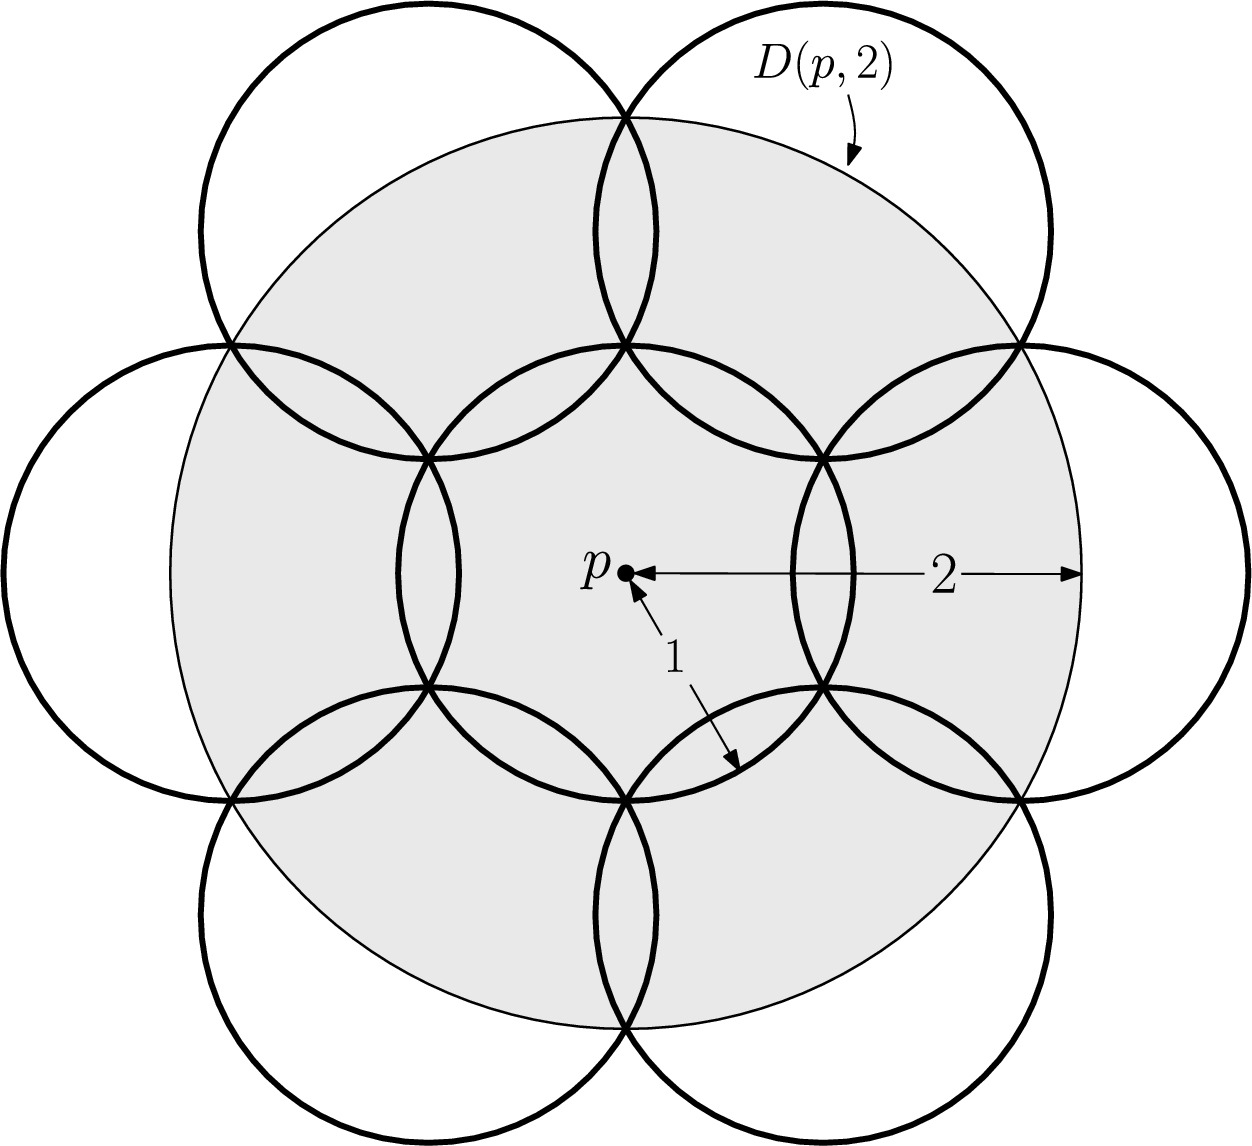
\includegraphics[width=0.4\textwidth]{figs/f1}
\caption{
پوشش $D(p,2)$ با دیسک‌های واحد
}
\label{fig:f1}
\end{figure}

در ادامه خواهید دید که چگونه می‌توان فاکتور تقریب را به 4 کاهش داد. $p$ را سمت چپ‌ترین نقطه در مجموعه $P$ درنظر بگیرید. در موارد خاص که مقادیر $x$ نقاط با هم برابر است، برای انتخاب سمت چپ‌ترین نقطه، کمتر بودن مقدار $y$ را ملاک قرار می‌دهیم. فرض کنید خط عمودی $l$ از نقطه $p$ عبور کند؛ $R(p)$ اشتراک $D(p,2)$ با نیم‌صفحه%
\LTRfootnote{Half-plane}
سمت راست $l$ خواهد بود؛ یعنی $R(p)$ نیم‌دیسک سمت راست $D(p,2)$ است (مطابق \cref{fig:f2}).

همان‌طور که قبلاً هم توضیح داده شد، تمام نقاط مجموعه $P$ که با $d(p)$ پوشش داده شده‌اند، در $D(p,2)$ و به‌تبع آن در $R(p)$ نیز قرار دارند. مطابق \cref{fig:f2}، نیم‌دیسک $R(p)$ می‌تواند با 4 دیسک واحد پوشش داده شود. قسمت دوم شکل، حالتی از موقعیت قرار گرفتن 7 نقطه را نشان می‌دهد که برای پوشش آنها حداقل به 4 دیسک واحد نیاز است.

\begin{figure}[!h]
\centering
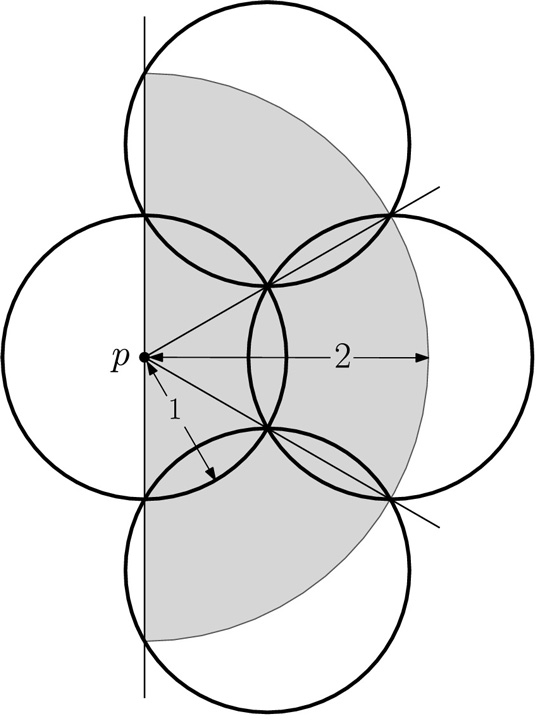
\includegraphics[width=0.3\textwidth]{figs/f2}
\caption{
پوشش $R(p)$ با دیسک‌های واحد
}
\label{fig:f2}
\end{figure}

برای نقطه‌ای مانند $p$ و مجموعه نقاط $I$ فاصله $d(p,I)$ برابر است با کمترین فاصله اقلیدسی بین $p$ و هر نقطه موجود در $I$ . اگر مجموعه $I$ تهی باشد، فاصله بینهایت درنظر گرفته می‌شود. \cref{blms1}، الگوریتم پیشنهادی با فاکتور تقریب 4 را نشان می‌دهد. خروجی آن، مجموعه‌ای از دیسک‌های واحد با نام $C$ است که مجموعه نقاط $P$ را پوشش می‌دهند. ابتدا لیستی از نقاط که از چپ به راست مرتب شده‌اند ایجاد می‌شود. سپس هردفعه اولین عنصر $p$ از لیست انتخاب و حذف می‌شود. اگر فاصله
$d(p,I) \leqslant 2$
باشد، نشان‌دهنده این است که قبلاً نقطه $p$ توسط یکی از دیسک‌های مجموعه $C$ پوشش داده شده است. در غیر این صورت، نیم‌دیسک $R(p)$ با 4 دیسک واحد پوشش داده می‌شود و به مجموعه $C$ اضافه می‌شود. در نهایت مجموعه دیسک‌های واحد $C$ به‌عنوان خروجی حاصل می‌شود.

\begin{algorithm}[!h]
\caption{
نسخه اولیه $BLMS$
}
\label{blms1}
\begin{latin}
\begin{algorithmic}[1]
%\REQUIRE A point set $P$ in the plane.
%\ENSURE A set $C$ of unit disks that cover $P$.
\STATE $C = \varnothing$
\STATE $I = \varnothing$
\STATE $L =$ List of points in $P$ sorted from left to right
\WHILE{$L$ is not empty}
    \STATE $p =$ first element of $L$
    \IF{$d(p,I) > 2$}
        \STATE Cover $R(p)$ by 4 unit disks $c_{1}, c_{2}, c_{3}, c_{4}$
        \STATE $C = C \cup \{ c_{1}, c_{2}, c_{3}, c_{4} \}$
        \STATE $I = I \cup \{ p \}$
    \ENDIF
    \STATE $L = L - \{ p \}$
\ENDWHILE
\STATE \textbf{return} $C$
\end{algorithmic}
\end{latin}
\end{algorithm}

در هر تکرار \cref{blms1} ، نقطه $p$ به مجموعه $I$ اضافه می‌شود، اگر و تنها اگر $d(p,I) > 2$ باشد. بنابراین $p$ در $UDIG(P)$ به هیچ نقطه‌ای از $I$ متصل نیست. همچنین بعد از خاتمه الگوریتم، $I$ یک مجموعه مستقل حداکثری خواهد بود.

\begin{theorem}
فاکتور تقریب \cref{blms1} برای مسئله پوشش دیسک واحد، 4 است.
\end{theorem}

\begin{cproof}
مجموعه نقاط $I$ و مجموعه دیسک‌های واحد $C$ را در پایان الگوریتم، درنظر بگیرید. براساس رابطه \ref{eq:1} می‌دانیم که نامساوی $|I| \leqslant |C^{*}|$ برقرار است. به‌ازای نقاط $p \in I$ هر نقطه $q \in P$ در یک نیم‌دیسک $R(p)$ قرار دارد (ممکن است $q = p$ باشد). چون برای هر نقطه $p \in I$ ، نیم‌دیسک $R(p)$ با 4 دیسک واحد پوشش داده می‌شود، مجموعه $C$ مجموعه $P$ را پوشش می‌دهد. بنابراین رابطه
$|C| \leqslant 4|I| \leqslant 4|C^{*}|$
برقرار است.
\end{cproof}

پیچیدگی زمانی \cref{blms1}
$O(n\log n + n.t(d))$
است. $t(d)$ پیچیدگی زمانی محاسبه فاصله $d(p,I)$ را نشان می‌دهد. محاسبه این فاصله با پیچیدگی زمانی $O(\log^{2}n)$ قابل انجام است \cite{bentley1980decomposable}. بنابراین پیچیدگی نهایی الگوریتم،
$O(\log^{2}n)$
است که در ادامه با استفاده از تکنیک جاروی صفحه، بهبود می‌یابد.

به‌جای محاسبه فاصله $d(p,I)$ کافی است بدانیم فاصله نقطه $p$ از مجموعه $I$ از 2 بیشتر است یا نه؛ یعنی به یک مسئله تصمیم‌گیری تبدیل شود. به‌تدریج که یک نقطه جدید مانند $p$ به مجموعه $I$ اضافه می‌شود، نقاط مجموعه $P$ که در نیم‌دیسک $R(p)$ قرار دارند، حذف می‌شوند. برهمین اساس، یک الگوریتم با استفاده از تکنیک جاروی صفحه و پیچیدگی زمانی $O(n\log n)$ ارائه می‌شود. 

در \cref{blms2}، ابتدا نقاط بر اساس مؤلفه $x$ از چپ به راست مرتب شده و در صف رخدادها درج می‌شوند. خط جارو به‌صورت عمودی از چپ به راست بر روی نقاط حرکت می‌کند. به هر نقطه که می‌رسد، اگر نقطه انتهایی یک نیم‌دیسک باشد، نقطه ابتدایی مربوط به آن نیم‌دیسک را از درخت وضعیت حذف می‌کند. در غیر این صورت، دو نقطه همسایه از بالا و دو نقطه همسایه از پایین را در درخت وضعیت برای این نقطه پیدا می‌کند. اگر فاصله آن با حداقل یکی از این 4 همسایه کمتر یا مساوی 2 باشد، به این معنا است که نقطه مورد نظر قبلاً در یک نیم‌دیسک قرار گرفته و تحت پوشش است و نیاز به اقدام خاصی نیست. در غیر این صورت، یک نیم‌دیسک به شعاع 2 و مرکز آن نقطه درنظر گرفته می‌شود و مرکز 4 دیسک واحد پوشش‌دهنده آن نیم‌دیسک محاسبه و به‌عنوان جواب گزارش می‌شود. سپس آن نقطه به‌عنوان نقطه ابتدایی نیم‌دیسک، در مکان مناسب خود در درخت وضعیت درج می‌شود. همچنین، نقطه انتهایی این نیم‌دیسک با اضافه کردن 2 واحد به مؤلفه $x$ مرکز آن، محاسبه شده و در جای مناسب در صف رخدادها درج می‌شود. لازم به ذکر است که درخت وضعیت، شامل نقاط ابتدایی نیم‌دیسک‌هایی است که در هر لحظه با خط جارو متقاطع‌اند و به‌صورت مرتب شده بر اساس مؤلفه $y$ از پایین به بالا قرار گرفته‌اند.


\begin{algorithm}[H]
\singlespacing
\caption{
نسخه بهبود یافته $BLMS$ با تکنیک جاروی صفحه
}
\label{blms2}
\begin{latin}
\begin{algorithmic}[1]
%\REQUIRE A point set $P$ in the plane.
%\ENSURE A set $C$ of unit disks that cover $P$.
\STATE Initialize an empty event queue $Q$. Insert the points in ascending order of their x-coordinates into $Q$.
\STATE Initialize an empty BST status structure $T$.
\STATE Initialize an empty list $C$.
\WHILE{$Q$ is not empty}
    \STATE Determine the next event point $p$ in $Q$ and delete it.
    \IF {$p$ is an end-point}
        \STATE Delete the start-point of the corresponding half-disk from $T$.
    \ELSE
        \STATE Find the 2 top and the 2 bottom neighbors of $p$ in $T$.
        \IF {The distance between $p$ and all of these 4 neighbors is greater than 2}
            \STATE Calculate center points of the 4 unit disks which cover half-disk of point $p$ and insert them into $C$.
            \STATE Insert $p$ into $T$.
            \STATE Insert the end-point $q=(p_x + 2, p_y)$ into $Q$.
        \ENDIF
    \ENDIF
\ENDWHILE
\STATE \textbf{return} $C$
\end{algorithmic}
\end{latin}
\end{algorithm}


\subsection{
الگوریتم $LL$
}

در این الگوریتم، صفحه به نوار‌های عمودی با عرض $\sqrt{3}$ تقسیم می‌شود. از هر نوار، یک جواب تقریبی با مرتب‌سازی نقاط براساس مؤلفه $y$ به‌صورت نزولی به‌دست می‌آید. نقطه بعدی درون یک نوار که هنوز پوشش داده نشده است، با قرار دادن یک دیسک در پایین‌ترین مکان ممکن، پوشش داده می‌شود. مرکز این دیسک‌ها، روی خطوط عمودی که نوارها را به دو قسمت تقسیم می‌کنند قرار می‌گیرد. جواب نهایی با اجتماع جوا‌ب همه نوارها حاصل می‌شود. این سامانه نواری، 5 مرتبه به سمت راست و هر دفعه به‌اندازه $\sqrt{3} / 6$ شیفت داده می‌شود. در هر شیف، یک جواب به‌دست می‌آید. از بین این 6 جواب، آن جوابی که کمترین دیسک را استفاده کرده باشد به‌عنوان جواب نهایی درنظر گرفته می‌شود. جزئیات بیشتر در
\cref{alg:LL}
موجود است. فاکتور تقریب این الگوریتم $25/6 \approx 4.17$ است.

\begin{algorithm}[H]
\singlespacing
\caption{
محاسبه موقعیت دیسک‌های واحد با استفاده از $LL$
} 
\label{alg:LL} 
\begin{latin}
\begin{algorithmic}[1] 
    \STATE $\textsc{Disk-Centers} \leftarrow \emptyset$, \texttt{min} $\leftarrow n+1$;
   
    \STATE Sort $P$ w.r.t $x$-coordinate in $O(n\log n)$ time;
\FOR{$i \in \{0,1,2,3,4,5\}$}

 \STATE \texttt{current} $\leftarrow 1$, $C \leftarrow \emptyset$, \texttt{right} $\leftarrow P[1]_x + \frac{i\sqrt{3}}{6}$;

 \WHILE{\texttt{current} $\leq n$}
     \STATE \texttt{index} $\leftarrow$ \texttt{current};
     
     \WHILE{$P[\texttt{current}]_x <$ right \textbf{and} \texttt{current} $\leq n$}
         \STATE \texttt{current} $\leftarrow$ \texttt{current} $+$ $1$;
     \ENDWHILE
     
     \STATE \texttt{$x$-of-restriction-line} $\leftarrow$ \texttt{right} $-\sqrt{3}/2$, \texttt{segments} $\leftarrow \emptyset$;
     
     \FOR{$j \leftarrow$ \texttt{index} \textbf{to} \texttt{current}$-1$}
         \STATE $d\leftarrow P[j]_x-$ \texttt{$x$-of-restriction-line}, $y\leftarrow \sqrt{1-d^2}$;
         \STATE Create a segment $s$ having the endpoints $(x\texttt{-of-restriction-line}, P[j]_y+y)$ and $(x\texttt{-of-restriction-line}, P[j]_y-y)$ and insert it into \texttt{segments};
     \ENDFOR
     
     \STATE Sort \texttt{segments} in non-ascending order based on $y$-coordinates of their tops. Greedily stab them by choosing the stabbing point as low as possible, while still stabbing the topmost unstabbed segment. Put the stabbing points (the disk centers) in $C$;
     
     \STATE Increment \texttt{right} by a multiple of $\sqrt{3}$ such that $P[\texttt{current}] - \texttt{right} \leq \sqrt{3}$;

 \ENDWHILE
 
   
     \IF{$|C| < $ \texttt{min}} 
         \STATE \textsc{Disk-Centers} $\leftarrow C$, \texttt{min} $\leftarrow |C|$;
     \ENDIF
\ENDFOR
\STATE \textbf{return} \textsc{Disk-Centers};
\end{algorithmic}
\end{latin}
\end{algorithm}



\subsection{
الگوریتم $DGT$
}

این الگوریتم، ساده و برخط است. به‌ازای هرنقطه‌ای که تاکنون تحت پوشش قرار نگرفته است، یک دیسک واحد به مرکز آن نقطه ایجاد می‌شود. فاکتور تقریب آن در صفحه، 5 است. در فضای با ابعاد $d$ دارای فاکتور تقریب $O(1.321^{d})$ است. برای مشاهده توصیف سطح بالا، به
\cref{alg:DGT}
مراجعه نمایید.

\begin{algorithm}[H]
\singlespacing
\caption{
محاسبه موقعیت دیسک‌های واحد با استفاده از $DGT$
} 
\label{alg:DGT} 
\begin{latin}
\begin{algorithmic}[1] 
   \STATE $\textsc{Disk-Centers} \leftarrow \emptyset$;
   \FOR{$p \in P$}
        \IF {the distance from $p$ to the nearest point in \textsc{Disk-Centers} is $>1$}
            \STATE \textsc{Disk-Centers} $\leftarrow$ \textsc{Disk-Centers} $\cup$ $\{p\}$; 
        \ENDIF
   \ENDFOR
   \STATE \textbf{return} \textsc{Disk-Centers};
   \end{algorithmic}
\end{latin}
\end{algorithm}


\subsection{
الگوریتم $FastCover$
}

در این الگوریتم، از یک شبکه%
\LTRfootnote{Grid}
با مربع‌های به ضلع $\sqrt{2}$ استفاده می‌شود. هر مربع از این شبکه، می‌تواند توسط یک دیسک به شعاع واحد محاط شود. به‌ازای هر نقطه، اگر توسط یکی از دیسک‌هایی که قبلاً قرار گرفته است تحت پوشش باشد، عملی انجام نمی‌شود؛ در غیر این صورت، یک دیسک واحد به مرکز مربعی که آن نقطه درونش قرار گرفته است، ایجاد می‌شود.

در پیاده‌سازی برای جستجوی سریع‌تر، از یک جدول درهم‌ساز%
\LTRfootnote{Hash table}
استفاده می‌شود. در این جدول، مختصات مرکز دیسک‌هایی که اضافه شده‌اند ذخیره می‌شود. برای جلوگیری از مشکلات اعداد اعشاری، از یک جفت عدد صحیح برای نمایش مرکز هر دیسک استفاده می‌شود. مختصات حقیقی می‌تواند با ضرب کردن هر عدد صحیح در $\sqrt{2}$ و اضافه کردن $\sqrt{2} / 2 = 1 / \sqrt{2}$ به آن به‌دست بیاید. برای به‌دست آوردن اعداد صحیح از روی یک نقطه، مؤلفه‌های $x,y$ آن بر $\sqrt{2}$ تقسیم می‌شود. درواقع این اعداد صحیح، مربع مربوط به آن نقطه را در شبکه نشان می‌دهد. این فرآیند در
\cref{alg:fastcover}
قابل ملاحظه است.

این الگوریتم دارای فاکتور تقریب 7 و پیچیدگی زمانی $O(n)$ است. یک الگوریتم برخط به‌حساب می‌آید و هیچ پیش‌پردازشی مثل مرتب‌سازی روی نقاط انجام نمی‌دهد. به‌اندازه $O(s)$ حافظه اضافی مصرف می‌کند که $s$ نشان‌دهنده اندازه پوشش تولید شده است.

\begin{algorithm}[H]
\singlespacing
\caption{
محاسبه موقعیت دیسک‌های واحد با استفاده از $FastCover$
} 
\label{alg:fastcover} 
\begin{latin}
\begin{algorithmic}[1] 
\STATE \texttt{$\mathcal{H}$} $\leftarrow \emptyset$; $\textsc{Disk-Centers} \leftarrow \emptyset$;
\FOR{$p \in P$}
\STATE  $i\leftarrow \lfloor p_x/\sqrt{2}\rfloor$;   $j\leftarrow \lfloor p_y/\sqrt{2}\rfloor$;

\IF{$(i,j) \notin \mathcal{H}$}
\STATE insert $(i,j)$ into $\mathcal{H}$ and  $(\sqrt{2}i + \frac{1}{\sqrt{2}}, \sqrt{2}j + \frac{1}{\sqrt{2}})$ into \textsc{Disk-Centers};
\ENDIF
\ENDFOR
\STATE \textbf{return} \textsc{Disk-Centers};
\end{algorithmic}
\end{latin}
\end{algorithm}


این الگوریتم را می‌توان کمی بهبود داد. وقتی که یک نقطه در یک مربع از شبکه قرار می‌گیرد، ممکن است توسط 4 دیسک واحد که مربوط به مربع‌های همسایه است و قبلاً اضافه شده‌اند تحت پوشش باشد (مطابق \cref{fig:f3}). بنابراین بهتر است برای کاهش تعداد دیسک‌ها این شرایط نیز بررسی شود. در
\cref{alg:fastcover+}
جزئیات نسخه بهبودیافته ذکر شده است.

\begin{figure}[H]
\centering
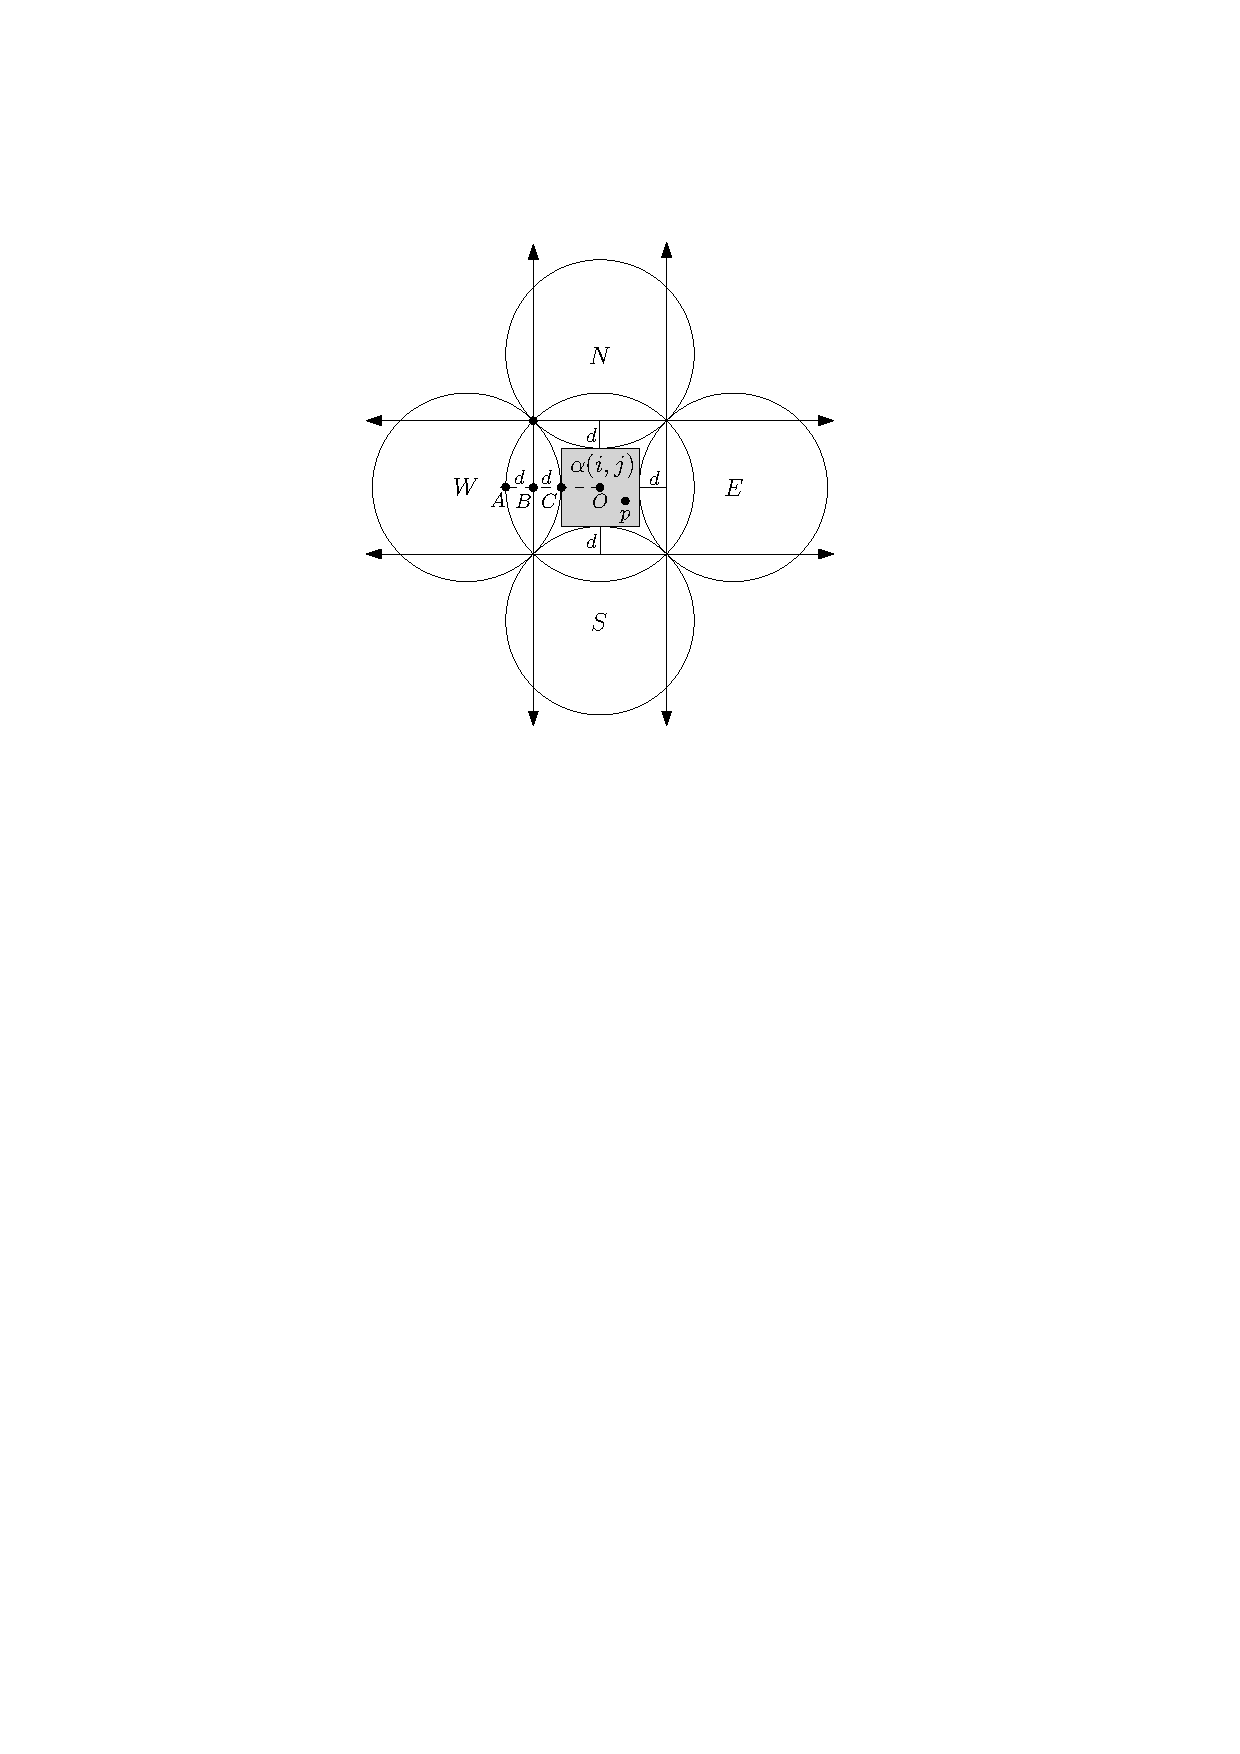
\includegraphics[width=0.4\textwidth]{figs/f3}
\caption{
امکان پوشش یک نقطه با دیسک‌های مربع‌های همسایه
}
\label{fig:f3}
\end{figure}


\begin{algorithm}[H]
\singlespacing
\caption{
محاسبه موقعیت دیسک‌های واحد با استفاده از $FastCover+$
} 
\label{alg:fastcover+} 
\begin{latin}	
	\begin{algorithmic}[1] 
		\STATE \texttt{$\mathcal{H}$} $\leftarrow \emptyset$;
		 $\textsc{Disk-Centers} \leftarrow \emptyset$;
		\FOR{$p \in P$}
		\STATE  $i\leftarrow \lfloor p_x/\sqrt{2}\rfloor$;  $j\leftarrow \lfloor p_y/\sqrt{2}\rfloor$;
		
		\IF{$(i,j) \in \mathcal{H}$}
		\STATE update $B(i,j)$ using $p$; \COMMENT{$p$ is already covered by $D(i,j)$}
		
			\ELSIF{$p_x \geq \sqrt{2}(i+1.5) -1$ \textbf{and} $({i}+1,{j}) \in\mathcal{H}$ \textbf{and} \\\quad $\texttt{distance}(p, (\sqrt{2}({i}+1)+\frac{1}{\sqrt{2}},\sqrt{2}{j}+\frac{1}{\sqrt{2}})) \leq 1$}
			\STATE \textbf{continue}; \COMMENT{$p$ is covered by the grid-disk $E$ placed before}
		
			\ELSIF{$p_x \leq \sqrt{2}(i-0.5)+1$ \textbf{and} $({i}-1,{j}) \in
				\mathcal{H}$ \textbf{and} \\\quad$\texttt{distance}(p, (\sqrt{2}({i}-1)+\frac{1}{\sqrt{2}},\sqrt{2}{j}+\frac{1}{\sqrt{2}})) \leq 1$}
			\STATE  \textbf{continue}; \COMMENT{$p$ is covered by the grid-disk $W$ placed before}
		
			\ELSIF{$p_y \geq \sqrt{2}(j+1.5) -1$ \textbf{and} $({i},{j+1}) \in
				\mathcal{H}$ \textbf{and}\\\quad $\texttt{distance}(p, (\sqrt{2}{i}+\frac{1}{\sqrt{2}},\sqrt{2}{(j+1)}+\frac{1}{\sqrt{2}})) \leq 1$}
			\STATE   \textbf{continue}; \COMMENT{$p$ is covered by the grid-disk $N$ placed before}
		
			\ELSIF{$p_y \leq \sqrt{2}(j-0.5)+1$ \textbf{and} $({i},{j-1}) \in
				\mathcal{H}$ \textbf{and} \\\quad$\texttt{distance}(p, (\sqrt{2}{i}+\frac{1}{\sqrt{2}},\sqrt{2}{(j-1)}+\frac{1}{\sqrt{2}})) \leq 1$}
			\STATE  \textbf{continue}; \COMMENT{$p$ is covered by the grid-disk $S$ placed before}
		
		\ELSE 
		\STATE insert $(i,j)$ into $\mathcal{H}$ and  $(\sqrt{2}i + \frac{1}{\sqrt{2}}, \sqrt{2}j + \frac{1}{\sqrt{2}})$ into \textsc{Disk-Centers};
		\ENDIF
		\ENDFOR
		\STATE \textbf{return} \textsc{Disk-Centers};
	\end{algorithmic}
\end{latin}
\end{algorithm}


بهبود دیگری می‌توان روی الگوریتم اعمال نمود. اگر نقاط موجود در دو دیسک مجاور را بتوان با یک دیسک پوشش داد، یعنی قطر مجموعه نقاط هر دو دیسک کمتر از 2 باشد، می‌توان آن دو دیسک را ادغام نمود. برای ادغام، یک دیسک واحد به مرکز وسط قطر مجموعه نقاط درنظر گرفته می‌شود. برای اینکه محاسبه قطر، تأثیری روی پیچیدگی زمانی الگوریتم نداشته باشد، به‌همراه هر دیسک واحدی که ایجاد می‌شود، یک مستطیل مرزی نیز برای مجموعه نقاط موجود در آن نگهداری می‌شود. هر دفعه که یک نقطه جدید تحت پوشش یک دیسک واحد قرار می‌گیرد، ابعاد مستطیل مرزی مربوط به آن نیز بروزرسانی می‌شود. این بروزرسانی در $O(1)$ قابل انجام است. جزئیات بیشتر در
\cref{alg:fastcover++}
ذکر شده است.


\begin{algorithm}[H]
\singlespacing
\caption{
محاسبه موقعیت دیسک‌های واحد با استفاده از $FastCover++$
} 
\label{alg:fastcover++} 
\begin{latin}
	\begin{algorithmic}[1] 
		\STATE \texttt{$\mathcal{H}$} $\leftarrow \emptyset$;
						 $\textsc{Disk-Centers} \leftarrow \emptyset$;

		\FOR{$p \in P$}
		\STATE  $i\leftarrow \lfloor p_x/\sqrt{2}\rfloor$;  $j\leftarrow \lfloor p_y/\sqrt{2}\rfloor$;
		
		\IF{$(i,j) \in \mathcal{H}$}
		\STATE update $B(i,j)$ using $p$; \COMMENT{$p$ is already covered by $D(i,j)$}
		
		\ELSIF{$p_x \geq \sqrt{2}(i+1.5) -1$ \textbf{and} $({i}+1,{j}) \in\mathcal{H}$ \textbf{and} \\\quad $\texttt{distance}(p, (\sqrt{2}({i}+1)+\frac{1}{\sqrt{2}},\sqrt{2}{j}+\frac{1}{\sqrt{2}})) \leq 1$}
		\STATE update $B(i+1,j)$ using $p$; \COMMENT{$p$ is covered by the grid-disk $E$ placed before}
		
		\ELSIF{$p_x \leq \sqrt{2}(i-0.5)+1$ \textbf{and} $({i}-1,{j}) \in
			\mathcal{H}$ \textbf{and} \\\quad$\texttt{distance}(p, (\sqrt{2}({i}-1)+\frac{1}{\sqrt{2}},\sqrt{2}{j}+\frac{1}{\sqrt{2}})) \leq 1$}
		\STATE  update $B(i-1,j)$ using $p$; \COMMENT{$p$ is covered by the grid-disk $W$ placed before}
		
		\ELSIF{$p_y \geq \sqrt{2}(j+1.5) -1$ \textbf{and} $({i},{j+1}) \in
			\mathcal{H}$ \textbf{and}\\\quad $\texttt{distance}(p, (\sqrt{2}{i}+\frac{1}{\sqrt{2}},\sqrt{2}{(j+1)}+\frac{1}{\sqrt{2}})) \leq 1$}
		\STATE   update $B(i,j+1)$ using $p$; \COMMENT{$p$ is covered by the grid-disk $N$ placed before}
		
		\ELSIF{$p_y \leq \sqrt{2}(j-0.5)+1$ \textbf{and} $({i},{j-1}) \in
			\mathcal{H}$ \textbf{and} \\\quad$\texttt{distance}(p, (\sqrt{2}{i}+\frac{1}{\sqrt{2}},\sqrt{2}{(j-1)}+\frac{1}{\sqrt{2}})) \leq 1$}
		\STATE   update $B(i,j-1)$ using $p$; \COMMENT{$p$ is covered by the grid-disk $S$ placed before}
		
		\ELSE 
		\STATE insert $(i,j)$ into $\mathcal{H}$ and initialize $B(i,j)$ using $p$;

		\ENDIF
		\ENDFOR

		\WHILE{there is a grid-disk $(i,j) \in \mathcal{H}$ that is not considered yet}
		\IF{there is a grid disk $(k,\ell) \in \mathcal{H}$ such that $|i-k|\leq 1, |j-\ell|\leq 1$ and the diagonal-length of the bounding-box $B:=B(i,j)\cup B(k,\ell)$ is at most $2$}
		\STATE remove $(i,j)$ and $(k,\ell)$ from $\mathcal{H}$ and 
	 add the center of $B$ to \textsc{Disk-Centers};
		\ENDIF
		\ENDWHILE
		
		\FOR{every grid-disk $(i,j) \in \mathcal{H}$}
		\STATE insert $(\sqrt{2}i + \frac{1}{\sqrt{2}}, \sqrt{2}j + \frac{1}{\sqrt{2}})$ into \textsc{Disk-Centers};
		\ENDFOR
		
		\STATE \textbf{return} \textsc{Disk-Centers};
	\end{algorithmic}
\end{latin}
\end{algorithm}



\section{ارزیابی}

همه الگوریتم‌ها با زبان $C++$ و کتابخانه $CGAL$ پیاده‌سازی شده‌اند. هرکدام از آنها بر روی 10 مجموعه‌نقطه دنیای واقعی اجرا شده‌اند.
\cref{tb:eval}
نتایج ارزیابی را نشان می‌دهد. هر الگوریتم، 5 بار بر روی هر مجموعه‌نقطه اجرا شده است. هر خانه کمترین تعداد دیسک و کمترین زمان پردازش برحسب ثانیه از بین این 5 اجرا را نشان می‌دهد. منظور از $LL-1P$ ، اجرای یک مرحله‌ای
\cref{alg:LL}
به‌جای شش مرحله است.

\begin{table}[H]
\centering
\singlespacing
\caption{
نتایج ارزیابی الگوریتم‌ها
} 
\label{tb:eval} 
\begin{latin}
\fontsize{8pt}{20pt}\selectfont
\begin{tabular}{|l|c|c|c|c|c|c|c|}
\hline
\multicolumn{1}{|c|}{\textbf{}} & LL & LL-1P & BLMS & DGT & FastCover & FastCover+ & FastCover++ \\ \hline
birch3 & 99989, 0.18 & 99991, 0.03 & 99994, 0.05 & 99993, 0.07 & 99996, 0.02 & 99995, 0.02 & 99980, 0.08 \\ \hline
monalisa & 100000, 0.15 & 100000, 0.03 & 100000, 0.11 & 100000, 0.08 & 100000, 0.02 & 100000, 0.02 & 100000, 0.08 \\ \hline
usa & 115475, 0.17 & 115475, 0.04 & 115475, 0.12 & 115475, 0.09 & 115475, 0.02 & 115475, 0.03 & 115475, 0.10 \\ \hline
KDDCU2D & 1147, 0.19 & 1152, 0.04 & 1692, 0.10 & 1626, 0.01 & 1418,    0.01 & 1374, 0.01 & 1257, 0.01 \\ \hline
europe & 168253, 0.35 & 168271, 0.06 & 168088, 0.19 & 168069, 0.16 & 168333, 0.03 & 168277, 0.04 & 167811, 0.20 \\ \hline
wildfires & 622, 3.74 & 622, 0.88 & 842, 1.21 & 787, 0.12 & 663, 0.04 & 637, 0.04 & 620, 0.06 \\ \hline
world & 6667, 2.84 & 6680, 0.51 & 9145, 0.79 & 10980, 0.15 & 7874, 0.03 & 7576, 0.04 & 6967, 0.07 \\ \hline
nyctaxi & 25, 13.84 & 26, 3.09 & 32, 2.90 & 31, 0.13 & 34, 0.05 & 31, 0.05 & 25, 0.10 \\ \hline
uber & 3, 21.06 & 3, 4.75 & 5, 4.03 & 5, 0.19 & 5, 0.06 & 4, 0.06 & 4, 0.16 \\ \hline
hail2015 & 888, 39.83 & 889, 9.82 & 1193, 11.19 & 1128, 0.74 & 901, 0.28 & 860, 0.28 & 847, 0.42 \\ \hline
\end{tabular}
\end{latin}
\end{table}


\section{نتیجه‌گیری}

در مجموعه‌نقطه‌های دنیای واقعی، اگر معیار با اهمیت‌تر برای ارزیابی، تعداد دیسک‌های استفاده شده باشد، الگوریتم $LL$ عملکرد بهتری دارد. هرچند که الگوریتم $FastCover^{++}$ در برخی موارد، هم از لحاظ تعداد دیسک‌ها و هم زمان اجرا، عملکرد بهتری داشته است.

اگر معیار مهم‌تر، زمان اجرا باشد الگوریتم $FastCover$ عملکرد بهتری داشته است؛ اما چون تفاوت چندانی با نسخه بهبودیافته خود که تعداد دیسک‌های کمتری تولید می‌کند ندارد، استفاده از $FastCover^{++}$ پیشنهاد می‌شود.

اگر هردو معیار تعداد دیسک‌ها و زمان اجرا با اهمیت باشد، استفاده از الگوریتم $FastCover^{++}$ توصیه می‌شود؛ چرا که تعادل خوبی بین هردو معیار برقرار می‌کند \cite{friederich2022experiments}.



\newpage
{
\fontsize{12pt}{10pt}\selectfont
\bibliographystyle{ieeetr-fa}
\bibliography{etc/references}
\addcontentsline{toc}{section}{مراجع}
}
\newpage



\section*{پیوست}
\addcontentsline{toc}{section}{پیوست}

همان‌طور که در
\cref{tb:1}
ملاحظه شد، بهترین الگوریتم‌هایی که تاکنون برای مسئله $UDC$ ارائه شده‌اند، دارای فاکتور تقریب 4 هستند. اینجانب، توجه زیادی به این مسئله با هدف بهبود فاکتور تقریب و نگارش مقاله نمودم. ایده‌های مختلفی برای بهبود فاکتور تقریب به ذهنم رسید که پس از بررسی‌های فراوان متوجه شدم برخی از آنها اشتباه است و برخی دیگر را به‌دلیل کمبود زمان نتوانستم به‌طور دقیق بررسی کنم. در ادامه تعدادی از آنها را بیان می‌کنم.

ایده اول، با هدف کاهش فاکتور تقریب از 4 به 3 بود. در
\cref{fig:f2}
نشان داده شد که برای پوشش یک نیم‌دیسک به شعاع 2، دقیقاً به 4 دیسک واحد احتیاج است. بر اساس این شکل، برای پوشش یک ربع‌دیسک نیز دقیقاً به 3 دیسک واحد احتیاج است. با فرض اینکه اشتراک دو نیم‌دیسک به شعاع 2 حداکثر با یک ربع‌دیسک قابل پوشش است، می‌توان یک‌بار مطابق
\cref{blms2}
خط جارو را از چپ به راست و بار دیگر از بالا به پایین حرکت داد. طی این دو مرحله، تعدادی نیم‌دیسک حاصل می‌شود. نواحی از نیم‌دیسک‌ها که با یکدیگر هم‌پوشانی پیدا می‌کنند (اشتراک نیم‌دیسک‌ها) مواردی است که لازم است با دیسک‌های واحد پوشش داده شود. پس از بررسی مشخص شد که این ایده عملی نیست. چون فرض اولیه اشتباه است و حالت‌هایی وجود دارد که اشتراک دو نیم‌دیسک بیشتر از حد تصور می‌شود و نمی‌توان آن را با یک ربع‌دیسک پوشش داد (مطابق \cref{fig:app1}).

\begin{figure}[!h]
\centering
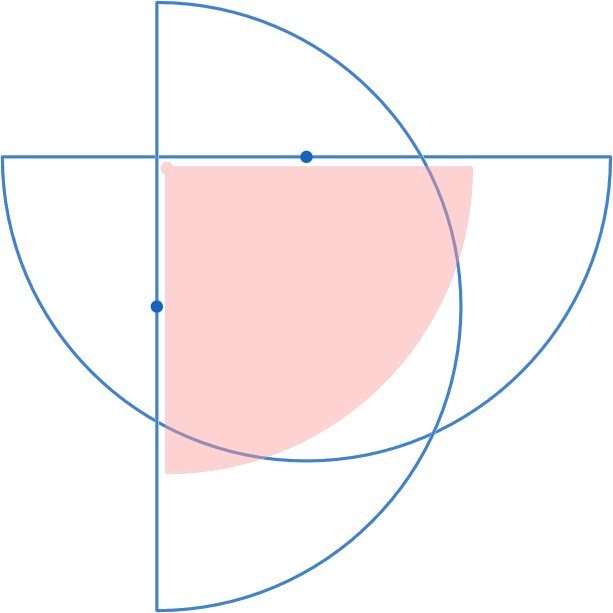
\includegraphics[width=0.3\textwidth]{figs/app1}
\caption{
عدم امکان پوشش اشتراک دو نیم‌دیسک با ربع‌دیسک
}
\label{fig:app1}
\end{figure}

ایده دوم نیز با هدف کاهش فاکتور تقریب از 4 به 3 بود. به‌جای نیم‌دیسک‌های با شعاع 2، ربع‌دیسک‌هایی به شعاع 2 درنظر گرفته می‌شود که هرکدام با 3 دیسک واحد قابل پوشش هستند. در
\cref{alg:app1}
جزئیات ایده بیان شده است. در این الگوریتم، خط جارو از بالا به پایین بر روی نقاط حرکت می‌کند. پس از بررسی، مشخص شد که این ایده نیز، عملی نیست. زیرا مانند
\cref{fig:app2}
حالت‌هایی وجود دارد که ربع‌دیسک‌های زیادی با یکدیگر همپوشانی پیدا می‌کنند و در نهایت فاکتور تقریب، $O(n)$ می‌شود.



\begin{algorithm}[H]
\singlespace
\caption{
ایده دوم برای کاهش فاکتور تقریب به 3 
}
\label{alg:app1}
\begin{latin}
\begin{algorithmic}[1]
%\REQUIRE A set $P$ of points in the plane.
%\ENSURE The set $C$ of Unit Disks which cover $P$.
\STATE Initialize an empty event queue $Q$. Insert the points in descending order of their y-coordinates into $Q$. If two points have the same y-coordinate, the one with smaller x-coordinate has higher priority.
\STATE Initialize an empty BST status structure $T$.
\STATE Initialize an empty list $C$.
\WHILE{$Q$ is not empty}
    \STATE Determine the next event point $p$ in $Q$ and delete it.
    \IF {$p$ is an end-point}
        \STATE Delete the start-point of the corresponding quarter disk from $T$.
    \ELSE
        \STATE Find the two left neighbors $p^{\prime}, p^{\prime \prime}$ of $p$ in $T$. If $p$ has the same x-coordinate with a point in $T$, consider the point with the higher y-coordinate as the left.
        \IF {$|pp^{\prime}| > 2$ and $|pp^{\prime \prime}| > 2$}
            \STATE Calculate center points of the 3 unit disks which cover quarter disk of point $p$ and insert them into $C$.
            \STATE Insert $p$ into $T$.
            \STATE Insert the end-point $q=(p_x, p_y + 2)$ into $Q$.
        \ENDIF
    \ENDIF
\ENDWHILE
\STATE \textbf{return} $C$
\end{algorithmic}
\end{latin}
\end{algorithm}


\begin{figure}[!h]
\centering
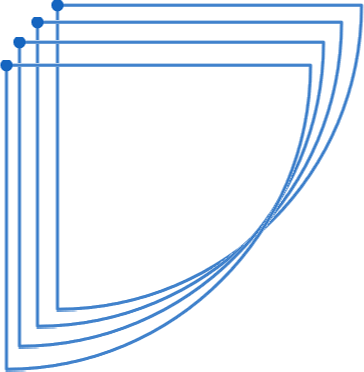
\includegraphics[width=0.25\textwidth]{figs/app2}
\caption{
حالتی که ربع‌دیسک‌های زیادی همپوشانی پیدا می‌کنند
}
\label{fig:app2}
\end{figure}


\end{document}
